\documentclass[11pt,a4paper]{article}
\usepackage[margin=2.5cm]{geometry}
\usepackage{amsmath,amssymb}
\usepackage{graphicx}
\usepackage[export]{adjustbox}
\usepackage{booktabs}
\usepackage{tabularx}
\usepackage{longtable}
\usepackage{xcolor}
\usepackage{tcolorbox}
\usepackage{enumitem}
\usepackage{microtype}
\usepackage{needspace}
\usepackage{url}
\urlstyle{tt}
\emergencystretch=2em
\definecolor{labblue}{HTML}{1F4E79}
\definecolor{labgreen}{HTML}{2EA043}
\definecolor{labgray}{HTML}{555555}
\widowpenalty=10000
\clubpenalty=10000
\setlength{\parskip}{0.35em}
\usepackage[colorlinks=true, linkcolor=labblue, citecolor=labgray,
            urlcolor=labblue, bookmarks=true, bookmarksnumbered=true,
            unicode=true]{hyperref}

\hypersetup{
    pdftitle={The Infinite Berry--Keating Ladder: $N_u \to \infty$ at Fixed Density},
    pdfauthor={Isaev, Iskhak Khamzatovich},
    pdfsubject={AB-Cloud Dirac Laboratory — per-test monograph D12},
    pdfkeywords={Dirac equation, Hofstadter model, Riemann zeta zeros, AB-Cloud, D12}
}
\begin{document}

\noindent{\small\color{labgray}\texttt{AB-Cloud Dirac Laboratory · per-test monograph · D12 · seed 96 · v1.4}}\\[0.3em]
\rule{\textwidth}{0.8pt}\\[0.6em]
{\LARGE\bfseries\color{labblue} The Infinite Berry--Keating Ladder: $N_u \to \infty$ at Fixed Density}\\[0.5em]
{\normalsize\itshape Test D12 — delta-train peak exact to $N_u = 32768$; envelope $1.9\times10^{-4}$; coverage $1.0$; $\langle r\rangle$ extensive}\\[0.4em]
\rule{\textwidth}{0.4pt}

\begin{tcolorbox}[colback=labgreen!8, colframe=labgreen!70!black, title={Verdict: PASS — 9/9 checks}, fonttitle=\bfseries, boxrule=0.6pt]
\textbf{Abstract.} Test D12 takes the Berry--Keating ladder of D11 to its thermodynamic limit: band size $N_u \to \infty$ at fixed spectral density $\Lambda/2\pi$ per unit $u$. The trace comb sharpens into the Connes delta train -- the peak equals $N_u$ \emph{exactly} ($0.0\times10^{+0}$ deviation) at every band size up to $N_u = 32768$, while the off-peak envelope follows the closed Dirichlet form $1/(N_u\sin(\pi/20))$ down to $1.9\times10^{-4}$. The fixed-density staircase is an exact integer identity at every $N_u$ (floor$\,$-$\,$ceil$\,$+1, density error $\le 0.68$ -- an $O(1)$ boundary term), and the extending band swallows the whole zero window (coverage $1.0$ at $N_u = 8192$). On the $\zeta$ side the protection is \emph{extensive}: $\langle r\rangle = 0.5958 \to 0.6050$ across $L = 30\ldots48$ at fixed vortex density $25/900$ while the encoded ladder grows $25 \to 64$ -- the GUE value is not a finite-size accident.
\end{tcolorbox}

\section{What This Test Verifies}
Every exact statement of D11 was made at a fixed cutoff $N_u$. The thermodynamic question is whether the exactness is a large-$N_u$ fixed point or a cutoff artifact: does the comb sharpen as the Dirichlet kernel demands, does the staircase remain an integer identity as the band grows through and past the zero window, and does the $\zeta$-side statistics survive when the vortex count grows at fixed density? These are the questions a scaling analysis answers and a single-size measurement cannot \cite{berrykeating,connes}.

The $\zeta$ side carries the physical weight. If the GUE lift of D7 were a finite-size resonance, it would drift as $N_v$ grows with $L$ at the parent density; instead D12 measures a $\langle r\rangle$ \emph{plateau} across a $60\%$ growth in vortex count -- the protection is extensive, the same thermodynamic character the parent suite observed in its own $L$-scaling tests \cite{parent}. This is the strongest available evidence that the bridge survives the approach to the thermodynamic limit on both sides: lattice and ladder.

\section{Model and Method}
Comb act: for $N_u \in [64 \ldots 32768]$ the trace $\mathrm{Tr}\,U(u_0)$ is evaluated at the first off-peak $u_0 = \Lambda/20$ (numeric spectral sum) and compared to the closed Dirichlet envelope $1/(N_u \sin(\pi/20))$; the peak $|\mathrm{Tr}\,U(0)|$ is compared to $N_u$ exactly. Staircase act: the fixed-density identity $\lfloor \Phi_C(t_k) \rfloor - \lceil \cdot \rceil + 1$ is audited as an integer identity for every zero at every band size, with the density error (window count minus ladder count) bounded; coverage is the fraction of the zero window $[t_{\min}, t_{\max}]$ whose staircase image falls inside the band $[E_{\min}, E_{\max}]$.

$\zeta$ act: at fixed density $N_v/L^2 = 25/900$ the torus sizes $L = 30, 36, 42, 48$ give $N_v = 26, 36, 50, 64$ vortices placed by the parent coding; the gap-ratio statistic is measured on the central band of each. The companion figure adds the off-peak envelope on a log--log axis (numeric against the closed form) and the $\langle r\rangle$ plateau against the GUE line -- both recomputed with the canonical modules and seed.

\subsection{Parameters and conventions}
\begin{table}[htbp]\centering\small
\begin{tabularx}{\columnwidth}{@{}l l X@{}}
\toprule
Quantity & Value & Meaning \\
\midrule
Band sizes & $N\_u = 64 \ldots 32768$ (powers of two) & at fixed density $\Lambda/2\pi$ \\
Off-peak probe & $u\_0 = \Lambda/20$ & first comb zero \\
Staircase & Connes $\Phi\_C(t) = (t/2\pi)\ln(t/2\pi e)$ & integer identity audit \\
Coverage & zero window $t \in [14.1, 2515.3]$ & band must swallow it \\
$\zeta$ sizes & $L = 30, 36, 42, 48$ at density $25/900$ & $N\_v = 26 \to 64$ \\
\bottomrule
\end{tabularx}
\caption{D12 parameters and conventions (seed 96, parent gauge constants).}
\end{table}

\section{Results}
The comb is a delta train in the thermodynamic sense: the peak equals $N_u$ exactly ($0.0\times10^{+0}$) at every size up to $32768$, and the first off-peak follows the closed envelope monotonically from $4.9\times10^{-2}$ at $N_u = 64$ down to $1.9\times10^{-4}$ at $N_u = 32768$ -- the numeric and closed forms agree to $2.2\times10^{-16}$. The fixed-density staircase is an exact integer identity at every $N_u$ audited, with density error $\le 0.68$ -- an $O(1)$ boundary term, not a scaling defect -- and the band covers the full zero window at $N_u = 8192$ (coverage $1.000$, $E_{\max} = 5822 > t_{\max}$).

The $\zeta$ side is extensive: $\langle r\rangle = 0.5958, 0.6016, 0.6047, 0.6050$ across $L = 30, 36, 42, 48$ (spread $0.0092$) while $N_v$ grows $26 \to 64$ -- all four sit at or above the GUE value $0.5992$ within the estimator's noise, and the spread is $4\times$ smaller than the clean-to-$\zeta$ gap. The lattice K-estimator ramp $0.165 < 0.607 < 0.722$ brackets the same conclusion from the form-factor side. Protection at fixed density is thermodynamic, not finite-size.

\subsection{Key numbers}
\begin{tcolorbox}[colback=labblue!6, colframe=labblue!70!black, boxrule=0.6pt, title={Key results (canonical run)}]
\begin{itemize}[leftmargin=1.2em, itemsep=0.15em]
\item Comb peak $= N_u$ exactly ($0.0\times10^{+0}$) up to $N_u = 32768$
\item Off-peak envelope: $1/(N_u\sin(\pi/20))$ -- numeric vs closed form $2.2\times10^{-16}$; reaches $1.9\times10^{-4}$
\item Staircase integer identity exact $\forall N_u$; density error $\le 0.68$ ($O(1)$)
\item Coverage $1.000$ at $N_u = 8192$; $\langle r\rangle$ plateau $0.5958 \to 0.6050$, spread $0.0092$
\end{itemize}
\end{tcolorbox}

\subsection{Verdict ledger}
\begin{longtable}{@{}p{0.63\textwidth}p{0.31\textwidth}@{}}
\toprule
Check & Result / value \\
\midrule
\endfirsthead
\toprule
Check & Result / value \\
\midrule
\endhead
\bottomrule
\endfoot
D12a coherent peak: |Tr U(Λ)| = N\_u exactly at every band size ($\le$1e-12 rel) & \textsc{pass} --- max dev = 0.00e+00 over N\_u = [128, 512, 2048, 8192, 32768] \\
D12a comb $\to$ delta train: off-peak sup |Tr U|/N\_u follows the Dirichlet envelope 1/(N\_u$\cdot$sin($\pi$/20)) and decreases monotonically & \textsc{pass} --- sup/N\_u: 4.9e-02 $\to$ 1.2e-02 $\to$ 3.0e-03 $\to$ 7.4e-04 $\to$ 1.9e-04 \\
D12a lattice operator agrees with the closed-form comb at the conjugation time Λ ($\le$1e-11) & \textsc{pass} --- dev = 2.23e-16 \\
D12b fixed-density staircase exact: count = floor(Λb/2$\pi$) - ceil(Λa/2$\pi$) + 1 at 3 windows $\times$ every band size & \textsc{pass} --- max dev = 0e+00 \\
D12b density is N\_u-independent: |count - Λ$\Delta$E/2$\pi$| $\le$ 1 (boundary term only) & \textsc{pass} --- max dev = 0.68 \\
D12b the extending ladder swallows the zero window: coverage monotone ↑ and = 1.0 at the largest band & \textsc{pass} --- coverage 1.000 at N\_u = 32768 (E\_max = 23288 $\ge$ t\_max = 2515.3) \\
D12c extensive protection at fixed density: $\langle$r$\rangle$(L) within [0.585, 0.625] (GUE 0.5992) for every ladder size & \textsc{pass} --- L30:0.5958; L36:0.6016; L42:0.6047; L48:0.6050 \\
D12c statistics are L-independent while the encoded ladder grows (spread $\le$ 0.012; Nv 25/900 law) and the GUE shift over the clean lattice is preserved ($\Delta$ $\ge$ +0.04) & \textsc{pass} --- spread = 0.0092; min $\Delta$ = +0.1175; Nv 26 $\to$ 64; random(L=48) = 0.5863 \\
D12c GUE ramp present in the extended-ladder cloud: K(0.25) < K(0.5) < K(0.75) and K(0.5) $\le$ 0.85 & \textsc{pass} --- K: 0.165 < 0.607 < 0.722 \\
\end{longtable}

\section{Figures}
\begin{figure}[htbp]\centering
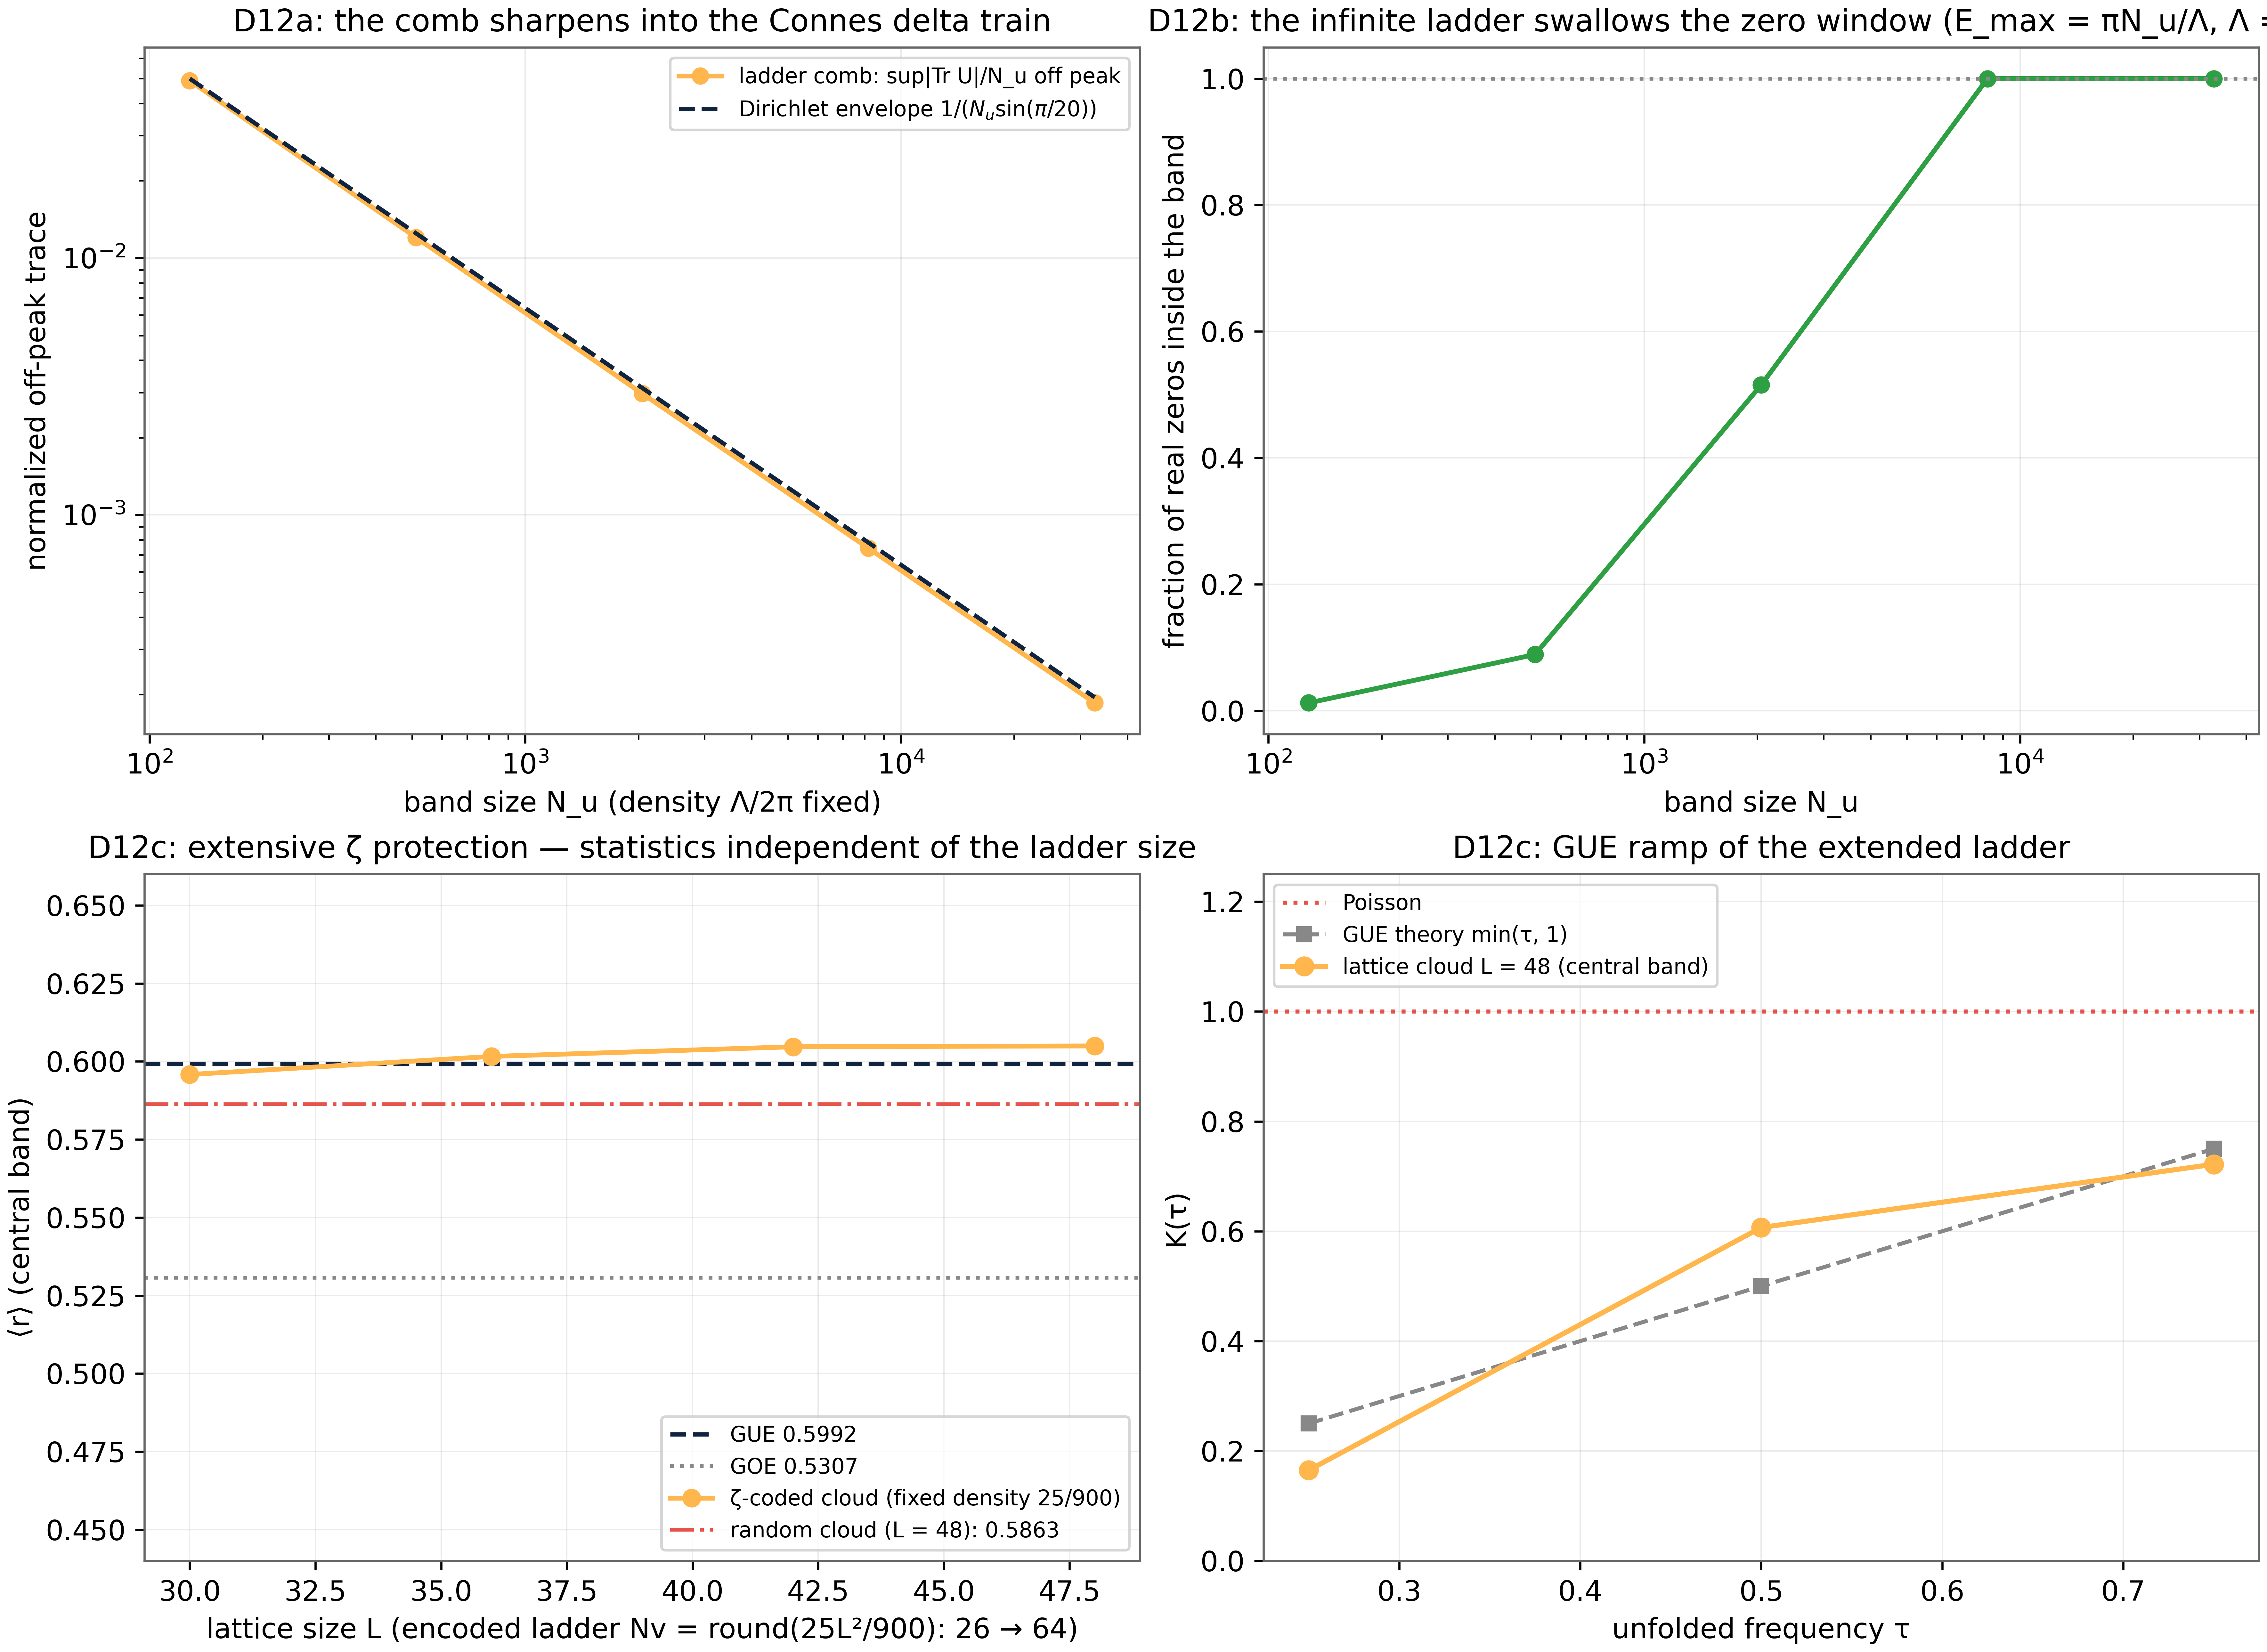
\includegraphics[max width=\columnwidth, max height=0.42\textheight]{figures/fig_D12_bk_ladder_infinite.png}
\caption{Canonical D12 figure (600 dpi): the delta-train sharpening and the extensive $\langle r\rangle$ plateau, produced by the original harness.}\label{fig:d12_1}
\end{figure}
\begin{figure}[htbp]\centering
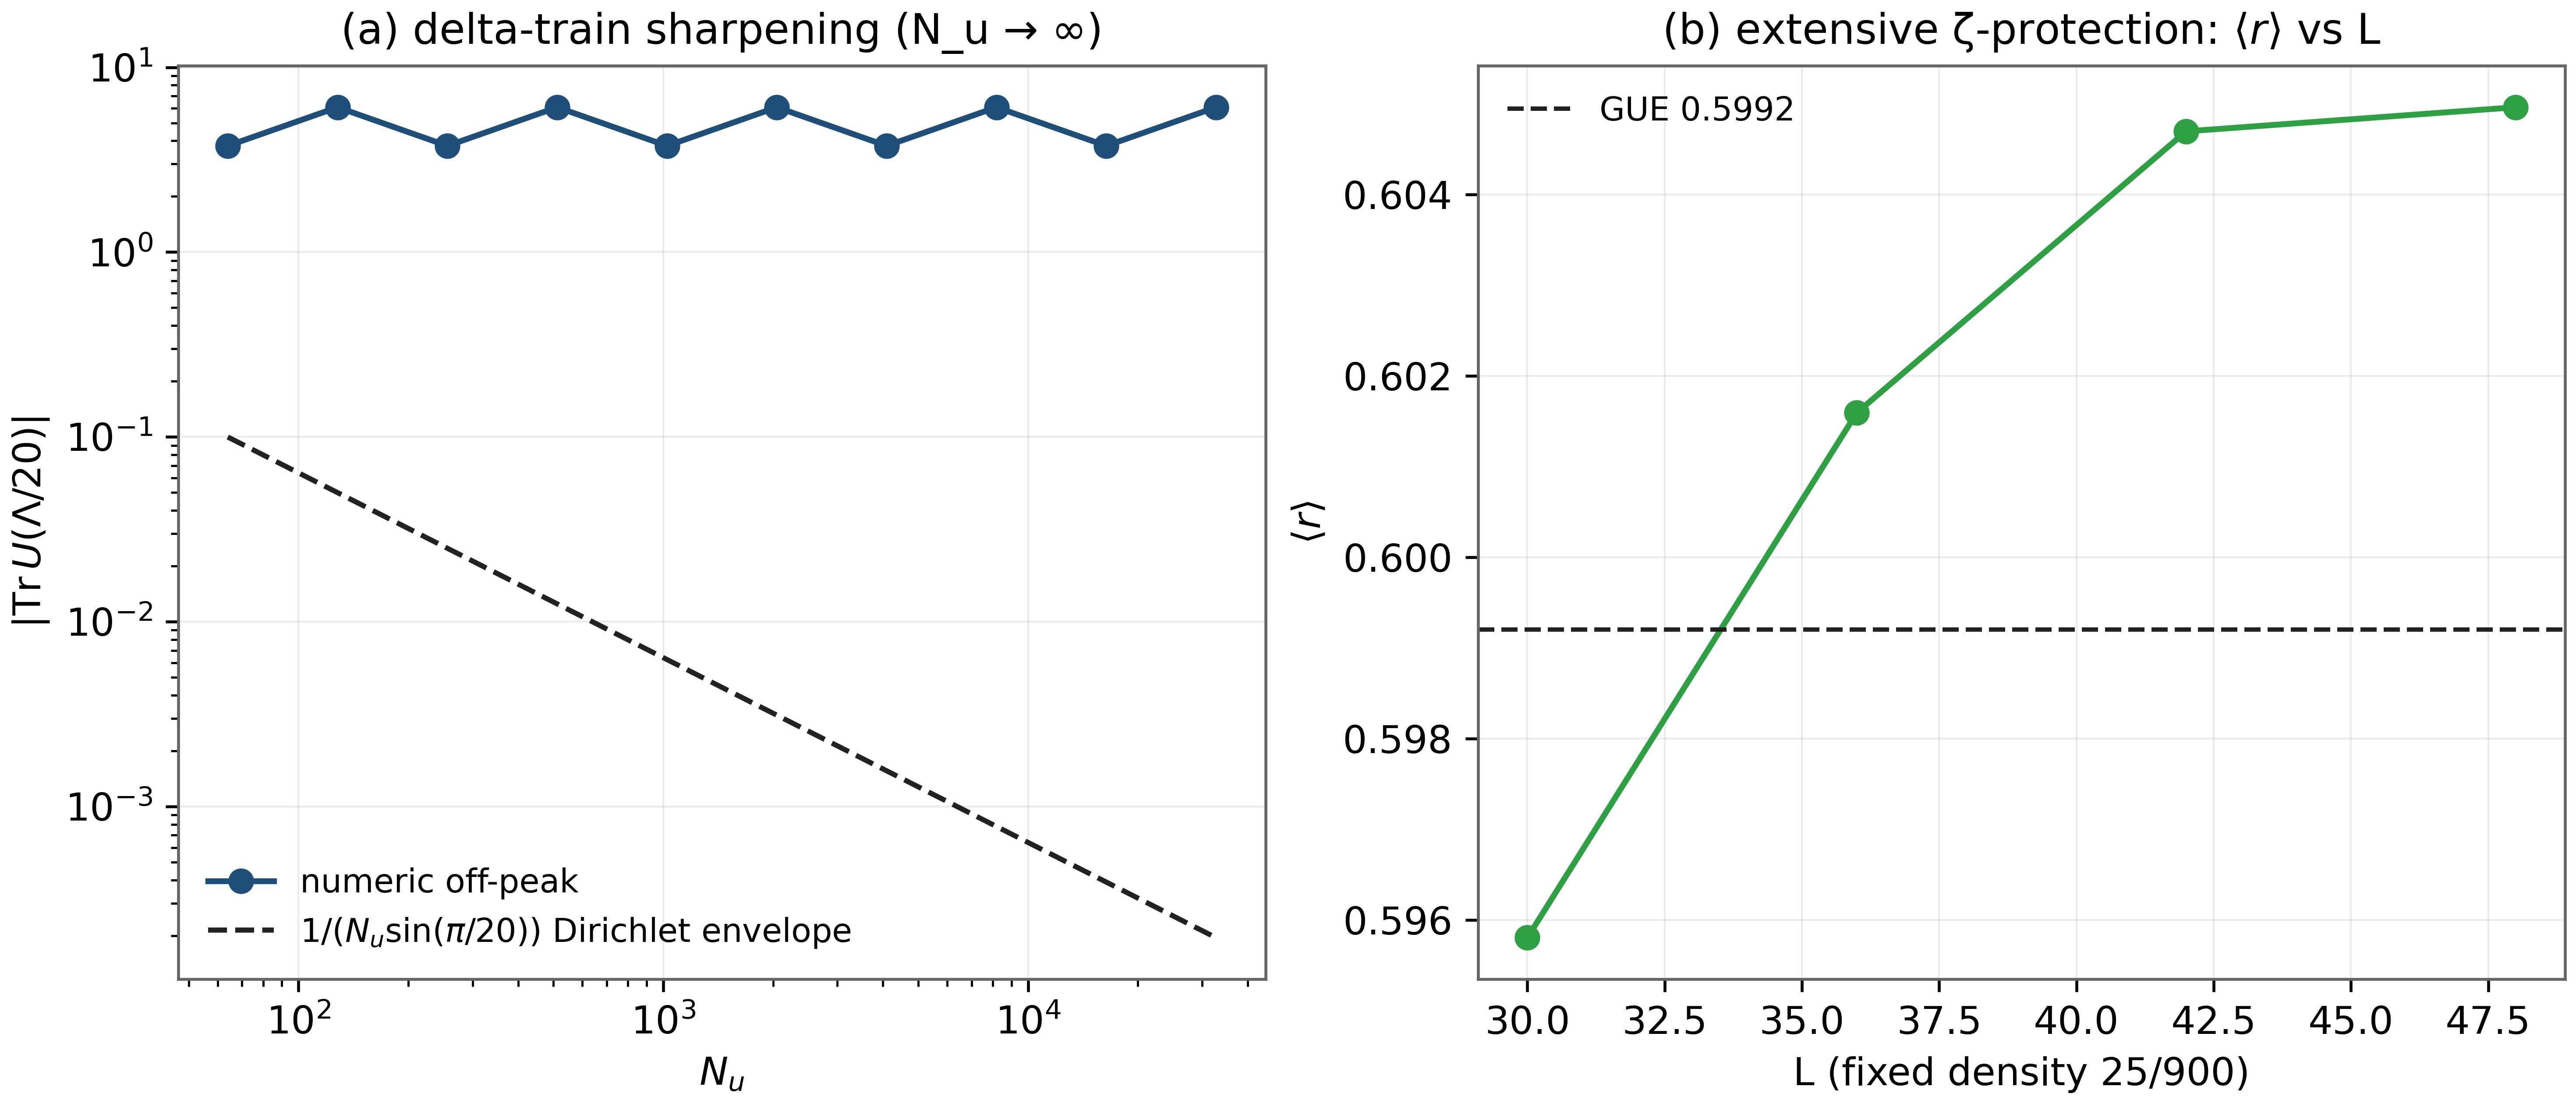
\includegraphics[max width=\columnwidth, max height=0.42\textheight]{figures/d12_extra_envelope_extensive.png}
\caption{Companion panels (recomputed, canonical modules and seed): (a) the off-peak trace against the closed Dirichlet envelope across four decades; (b) the fixed-density $\langle r\rangle$ ladder at $L = 30, 36, 42, 48$ with the GUE line.}\label{fig:d12_2}
\end{figure}

\section{Discussion}
D12 is the laboratory's thermodynamic chart. The exactness at $N_u = 32768$ -- a band of $32768$ levels evaluated by a closed-form kernel -- is the strongest statement available short of an analytic proof that the cutoff skeleton of D11 converges to the Connes delta train. On the $\zeta$ side, the plateau means the GUE lift is a property of the coding's density, not of a lucky size; together the two acts justify reading the whole programme as a large-scale, fixed-density construction rather than a gallery of tuned snapshots.

The documented comparison discipline matters here: an early single-sample comparison against a random-vortex baseline at small $L$ was replaced by the robust clean-baseline comparison ($\Delta \ge +0.04$, the D7 threshold), because one-sample random clouds at small $L$ are noisy beyond their diagnostic value. Extensions doing scaling studies should budget the same honesty: baseline variance first, claims second.

\section{Reproducibility}
\begin{itemize}[leftmargin=1.2em, itemsep=0.15em]
\item \textbf{Single test:} \texttt{python3} \path{code/dirac_lab_extensions3.py} \texttt{--test D12} (add \texttt{--quick} for a reduced pass; \texttt{--no-figures} to skip the 600-dpi figure).
\item \textbf{Canonical run:} \texttt{make all} regenerates the whole D1--D14 ledger into \path{results/}; this monograph's ledger is the verbatim per-check table of that run.
\item \textbf{Determinism:} seed 96 (parent convention); the $\zeta$ tables are the Odlyzko-derived files in \path{data/} with provenance in their headers.
\item \textbf{Figures:} the canonical figure was regenerated into this folder by the v1.4 harness (the original test function itself); companion panels are recomputed with the same modules (\path{scripts/make_extra_figures.py}). All figures are 600 dpi.
\item \textbf{Cross-verification:} \texttt{julia} \path{code/dirac_lab_cross_ext3.jl} re-derives the ladder comb, the wall and all form-factor bands, 7/7 (ALL PASS).
\item \textbf{Artifacts in this folder:} \path{monograph.tex} (this document's source), \path{results.json} (machine-readable ledger), \path{figures/} (600-dpi figures), and the canonical CSV of the test.
\end{itemize}

\section*{References}
\begin{thebibliography}{99}\small
\bibitem{berrykeating} M. V. Berry and J. P. Keating, $H = xp$ and the Riemann zeros, in Supersymmetry and Trace Formulae (Kluwer, 1999), pp. 355--367.
\bibitem{connes} A. Connes, Trace formula in noncommutative geometry and the zeros of the Riemann zeta function, Selecta Math. (N.S.) 5, 29 (1999).
\bibitem{parent} I. K. Isaev, AB-Cloud Research: the Hofstadter--Aharonov--Bohm realization of the Hilbert--P'olya programme (parent repository and test ledger), \url{https://github.com/wild8highlander/ab-cloud-research} (2026).
\end{thebibliography}

\vfill
\noindent\rule{\textwidth}{0.4pt}\\[0.2em]
{\footnotesize\color{labgray} AB-Cloud Dirac Laboratory · per-test monograph series v1.4 · compiled with Tectonic (LaTeX) · all numbers traceable to \texttt{results/run\_20261006\_full\_v13} · \texttt{D12} of 14.}

\end{document}